% Options for packages loaded elsewhere
\PassOptionsToPackage{unicode}{hyperref}
\PassOptionsToPackage{hyphens}{url}
%
\documentclass[
]{book}
\usepackage{lmodern}
\usepackage{amssymb,amsmath}
\usepackage{ifxetex,ifluatex}
\ifnum 0\ifxetex 1\fi\ifluatex 1\fi=0 % if pdftex
  \usepackage[T1]{fontenc}
  \usepackage[utf8]{inputenc}
  \usepackage{textcomp} % provide euro and other symbols
\else % if luatex or xetex
  \usepackage{unicode-math}
  \defaultfontfeatures{Scale=MatchLowercase}
  \defaultfontfeatures[\rmfamily]{Ligatures=TeX,Scale=1}
\fi
% Use upquote if available, for straight quotes in verbatim environments
\IfFileExists{upquote.sty}{\usepackage{upquote}}{}
\IfFileExists{microtype.sty}{% use microtype if available
  \usepackage[]{microtype}
  \UseMicrotypeSet[protrusion]{basicmath} % disable protrusion for tt fonts
}{}
\makeatletter
\@ifundefined{KOMAClassName}{% if non-KOMA class
  \IfFileExists{parskip.sty}{%
    \usepackage{parskip}
  }{% else
    \setlength{\parindent}{0pt}
    \setlength{\parskip}{6pt plus 2pt minus 1pt}}
}{% if KOMA class
  \KOMAoptions{parskip=half}}
\makeatother
\usepackage{xcolor}
\IfFileExists{xurl.sty}{\usepackage{xurl}}{} % add URL line breaks if available
\IfFileExists{bookmark.sty}{\usepackage{bookmark}}{\usepackage{hyperref}}
\hypersetup{
  pdftitle={Advance Mathematic MCOMD0AMA},
  pdfauthor={Dr.~Alexios Louridas},
  hidelinks,
  pdfcreator={LaTeX via pandoc}}
\urlstyle{same} % disable monospaced font for URLs
\usepackage{color}
\usepackage{fancyvrb}
\newcommand{\VerbBar}{|}
\newcommand{\VERB}{\Verb[commandchars=\\\{\}]}
\DefineVerbatimEnvironment{Highlighting}{Verbatim}{commandchars=\\\{\}}
% Add ',fontsize=\small' for more characters per line
\usepackage{framed}
\definecolor{shadecolor}{RGB}{248,248,248}
\newenvironment{Shaded}{\begin{snugshade}}{\end{snugshade}}
\newcommand{\AlertTok}[1]{\textcolor[rgb]{0.94,0.16,0.16}{#1}}
\newcommand{\AnnotationTok}[1]{\textcolor[rgb]{0.56,0.35,0.01}{\textbf{\textit{#1}}}}
\newcommand{\AttributeTok}[1]{\textcolor[rgb]{0.77,0.63,0.00}{#1}}
\newcommand{\BaseNTok}[1]{\textcolor[rgb]{0.00,0.00,0.81}{#1}}
\newcommand{\BuiltInTok}[1]{#1}
\newcommand{\CharTok}[1]{\textcolor[rgb]{0.31,0.60,0.02}{#1}}
\newcommand{\CommentTok}[1]{\textcolor[rgb]{0.56,0.35,0.01}{\textit{#1}}}
\newcommand{\CommentVarTok}[1]{\textcolor[rgb]{0.56,0.35,0.01}{\textbf{\textit{#1}}}}
\newcommand{\ConstantTok}[1]{\textcolor[rgb]{0.00,0.00,0.00}{#1}}
\newcommand{\ControlFlowTok}[1]{\textcolor[rgb]{0.13,0.29,0.53}{\textbf{#1}}}
\newcommand{\DataTypeTok}[1]{\textcolor[rgb]{0.13,0.29,0.53}{#1}}
\newcommand{\DecValTok}[1]{\textcolor[rgb]{0.00,0.00,0.81}{#1}}
\newcommand{\DocumentationTok}[1]{\textcolor[rgb]{0.56,0.35,0.01}{\textbf{\textit{#1}}}}
\newcommand{\ErrorTok}[1]{\textcolor[rgb]{0.64,0.00,0.00}{\textbf{#1}}}
\newcommand{\ExtensionTok}[1]{#1}
\newcommand{\FloatTok}[1]{\textcolor[rgb]{0.00,0.00,0.81}{#1}}
\newcommand{\FunctionTok}[1]{\textcolor[rgb]{0.00,0.00,0.00}{#1}}
\newcommand{\ImportTok}[1]{#1}
\newcommand{\InformationTok}[1]{\textcolor[rgb]{0.56,0.35,0.01}{\textbf{\textit{#1}}}}
\newcommand{\KeywordTok}[1]{\textcolor[rgb]{0.13,0.29,0.53}{\textbf{#1}}}
\newcommand{\NormalTok}[1]{#1}
\newcommand{\OperatorTok}[1]{\textcolor[rgb]{0.81,0.36,0.00}{\textbf{#1}}}
\newcommand{\OtherTok}[1]{\textcolor[rgb]{0.56,0.35,0.01}{#1}}
\newcommand{\PreprocessorTok}[1]{\textcolor[rgb]{0.56,0.35,0.01}{\textit{#1}}}
\newcommand{\RegionMarkerTok}[1]{#1}
\newcommand{\SpecialCharTok}[1]{\textcolor[rgb]{0.00,0.00,0.00}{#1}}
\newcommand{\SpecialStringTok}[1]{\textcolor[rgb]{0.31,0.60,0.02}{#1}}
\newcommand{\StringTok}[1]{\textcolor[rgb]{0.31,0.60,0.02}{#1}}
\newcommand{\VariableTok}[1]{\textcolor[rgb]{0.00,0.00,0.00}{#1}}
\newcommand{\VerbatimStringTok}[1]{\textcolor[rgb]{0.31,0.60,0.02}{#1}}
\newcommand{\WarningTok}[1]{\textcolor[rgb]{0.56,0.35,0.01}{\textbf{\textit{#1}}}}
\usepackage{longtable,booktabs}
% Correct order of tables after \paragraph or \subparagraph
\usepackage{etoolbox}
\makeatletter
\patchcmd\longtable{\par}{\if@noskipsec\mbox{}\fi\par}{}{}
\makeatother
% Allow footnotes in longtable head/foot
\IfFileExists{footnotehyper.sty}{\usepackage{footnotehyper}}{\usepackage{footnote}}
\makesavenoteenv{longtable}
\usepackage{graphicx,grffile}
\makeatletter
\def\maxwidth{\ifdim\Gin@nat@width>\linewidth\linewidth\else\Gin@nat@width\fi}
\def\maxheight{\ifdim\Gin@nat@height>\textheight\textheight\else\Gin@nat@height\fi}
\makeatother
% Scale images if necessary, so that they will not overflow the page
% margins by default, and it is still possible to overwrite the defaults
% using explicit options in \includegraphics[width, height, ...]{}
\setkeys{Gin}{width=\maxwidth,height=\maxheight,keepaspectratio}
% Set default figure placement to htbp
\makeatletter
\def\fps@figure{htbp}
\makeatother
\setlength{\emergencystretch}{3em} % prevent overfull lines
\providecommand{\tightlist}{%
  \setlength{\itemsep}{0pt}\setlength{\parskip}{0pt}}
\setcounter{secnumdepth}{5}
\usepackage{booktabs}
\usepackage[]{natbib}
\bibliographystyle{apalike}

\title{Advance Mathematic MCOMD0AMA}
\author{Dr.~Alexios Louridas}
\date{2021-02-06}

\begin{document}
\maketitle

{
\setcounter{tocdepth}{1}
\tableofcontents
}
\hypertarget{introduction}{%
\chapter*{Introduction}\label{introduction}}
\addcontentsline{toc}{chapter}{Introduction}

\hypertarget{module-structure}{%
\section*{Module Structure}\label{module-structure}}
\addcontentsline{toc}{section}{Module Structure}

We are going to have 12 weeks of teaching. What we would like at the end of this module is for you to be able to have enough knowledge to be able to understand mathematics so you can easily understand concepts that you will find in your course that you are going to follow.

Mathematics is not just about learning how to solve problems but

The indicative schedule we are going to follow can be seen in table 0.1. Although we shall try and follow this schedule it all depends on you. If you believe that you need an extra session to describe and master something then we are here to listen. Please tell us and we shall try to change it accordingly.

\begin{table}

\caption{\label{tab:unnamed-chunk-1}Indicative Content Schedule.}
\centering
\begin{tabular}[t]{c|c}
\hline
Session & Indicative Content\\
\hline
0 & Numbers\\
\hline
1 & Algebra - Basics\\
\hline
2 & Algebra - Quadratics and Simultaneous Equations\\
\hline
3 & Geometry and thinking\\
\hline
4 & Graphs and Coordinate Geometry\\
\hline
5 & Probability and Statistics\\
\hline
6 & Polynomials\\
\hline
7 & Logarithms and Exponential\\
\hline
8 & Introduction to Discrete Mathematics\\
\hline
9 & Systems\\
\hline
10 & Summary and Revision, TCA\\
\hline
11 & Assignment\\
\hline
\end{tabular}
\end{table}

\hypertarget{assignment}{%
\section*{Assignment}\label{assignment}}
\addcontentsline{toc}{section}{Assignment}

TCA 40\%
The TCA will consist of a series of tasks, each examining one area of mathematics.

The second assessment will be a group report and will consist of individual tasks that would be needed to be placed together to produce an end group report.

\hypertarget{numbers}{%
\chapter{Numbers}\label{numbers}}

This chapter will introduce you to numbers and their significance in mathematics and computing.
Since the beginning of humanity numbers were used to be able to count. The first evidence found that humans were counting was discovered in 1970 by \emph{Peter Beaumont} near the Lebombo Mountains. The artifact was a baboon fibula that had 29 straight cuts (see figure 1.1). It is hypothesised that it was used to count the menstrual cycles of women. Thus, it can be said that the first astronomers / mathematicians were women.

\begin{figure}

{\centering 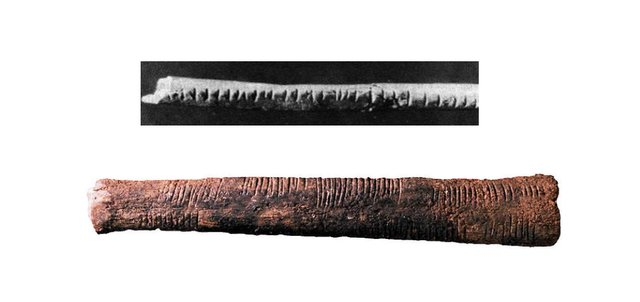
\includegraphics[width=1\linewidth]{images/Lebombo-bone} 

}

\caption{The Lebombo bone 44, 000 BC (top) and the Ishango bone 20, 000 BC (bottom)}\label{fig:unnamed-chunk-2}
\end{figure}

Numbers were and still are used to advance our civilization, from computing to art and music. From simple counting we have used numbers to calculate and measure. To achieve thought all of these advancements different types of numbers have been used, each having its own usage.

\hypertarget{types-of-number}{%
\section{Types of Number}\label{types-of-number}}

\hypertarget{number-zero}{%
\subsection{Number Zero}\label{number-zero}}

Zero as a mathematical symbol has a turbulence timeline. Although its first appearance was first seen by the Sumerians in Mesopotamia, some 5,000 years ago, it was used very infrequently by the Greeks and nothing has been found about the notion of zero by the Romans. On the other hand it has been seen by the Myans, Hindus, Chinese, but the way we use it today and its notions first appeared in the 20th century.

\hypertarget{natural-numbers-n}{%
\subsection{Natural Numbers (N)}\label{natural-numbers-n}}

One of the oldest and familiar number type are the natural numbers \(N\).
Natural numbers are used for counting and in arithmetic calculations. These include all whole numbers from 1 to infinity \(\infty\)

\begin{figure}

{\centering 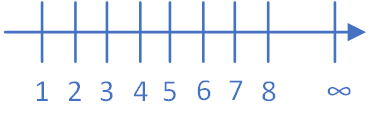
\includegraphics[width=0.4\linewidth]{images/Natural Numbers} 

}

\caption{Natural Numbers}\label{fig:unnamed-chunk-3}
\end{figure}

\hypertarget{whole-numbers-w}{%
\subsection{Whole Numbers (W)}\label{whole-numbers-w}}

The most common numbers used are for counting and are used in arithmetic calculations. These are whole numbers from 1 to infinity and zero.

\begin{figure}

{\centering 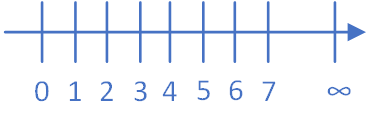
\includegraphics[width=0.4\linewidth]{images/Whole Numbers} 

}

\caption{Whole Numbers}\label{fig:unnamed-chunk-4}
\end{figure}

\hypertarget{integer-numbers-z}{%
\subsection{Integer Numbers (Z)}\label{integer-numbers-z}}

Another important set of numbers, especially for computing, are all whole numbers including negative whole numbers.These numbers are called Integer numbers and the range covered are all integer numbers from negative infinity to zero and from zero to positive infinity.

\begin{figure}

{\centering 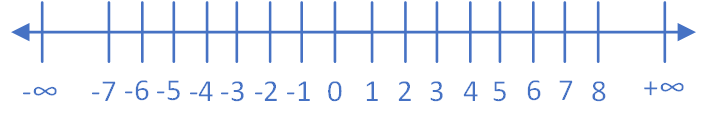
\includegraphics[width=0.6\linewidth]{images/Integer Numbers} 

}

\caption{Integer Numbers}\label{fig:unnamed-chunk-5}
\end{figure}

In computer programming these are the most used number set, as they are used in \emph{loops} as well as determining locations in memory. These are the numbers that are more efficient to be processed by a CPU and thus in many situation developers would prefer to use integer maths for effciency.

A significant property of integers is that when two integers are added, subtracted, or multiplied, the result is always another integer. However, when an integer is divided by another integer, the result can either be an integer or a fraction. This is very important especially in computing as a division of integers would change the type of variable you are using.

\hypertarget{rational-numbers-q}{%
\subsection{Rational Numbers (Q)}\label{rational-numbers-q}}

All numbers that can be expressed as a fraction (ratio) of integers are called rational numbers, as long as the denominator is not zero. So, rational numbers include all integer numbers as all integer number can be divided by 1 and become a fraction.

\hypertarget{irrantional-numbers-rq}{%
\subsection{Irrantional Numbers (R\textbackslash Q)}\label{irrantional-numbers-rq}}

In computer science, it is significant if a number is rational or irrational. A rational number can be stored as an exact numeric value, while an irrational number must be estimated.

When dealing with rational numbers in computing these could be easily stored as two integers, but when dealing with irrational numbers usually an estimation is necessary.
An example of that is the irrational number of the mathematical constant \(\pi\). This constant is the ratio of the circumference of any circle to the diameter of that circle, regardless of the circle's size. The number of digits for \(\pi\) are infinite \(\infty\) and it would be impossible to store a number with unlimited digits, so it often estimate to be \(3.14\).

\hypertarget{real-numbers-r}{%
\subsection{Real Numbers (R)}\label{real-numbers-r}}

If we include all rational and irrational numbers we get another in a set we get another set called real numbers.
This number set is the most common and used by everyone, as it include all numbers.

\hypertarget{complex-numbers-c}{%
\subsection{Complex Numbers (C)}\label{complex-numbers-c}}

When dealing with measuring or counting, real numbers are sufficient to describe what we want. When though we are trying to describe more than one dimension we find that real numbers are not enough and complicate measurements and calculations when trying to define or understand some of the notions of a point in space. The solution is to use multi-dimensional numbers, and through this it was found that besides real numbers there are also imaginary numbers. Imaginary numbers are nothing else that the multiplication of a real number to the ``unit'' of the imaginary number. The ``unit'' is the square root of -1 \(\sqrt-1\).
Complex numbers are all numbers that have a single real number and a single imaginary number.

\hypertarget{algebraic-properties}{%
\section{Algebraic Properties}\label{algebraic-properties}}

In this module we are going to be dealing mostly with real numbers, besides some exceptions. Thus, it would be good to know some of the basic algebraic properties of real numbers.

\hypertarget{closure}{%
\subsection{Closure}\label{closure}}

When adding or multiplying two real numbers the result is always a real number.
\(a + b\) and \(ab\) are always real numbers if \(a\) and \(b\) are real numbers.

\hypertarget{commutative}{%
\subsection{Commutative}\label{commutative}}

While adding or multiplying real numbers the position of the numbers do not alter the result.

\(a + b + c = b + a + c = a + c + b\)

similarly,

\(abc = cba\)

\begin{verbatim}
_Addition_
24 + 42 + 23 + 55 = 144   

can also be written as

42 + 23 + 55 + 24 = 144   

or

55 + 42 + 24 + 23 = 144   

_Multiplication_
10 * 24 * 2 = 480

can also be written as

2 * 24 * 10 = 480

or

24 * 2 * 10 = 480
\end{verbatim}

\hypertarget{associative}{%
\subsection{Associative}\label{associative}}

When adding or multiplying real numbers, grouping does not have an effect on the result. By grouping we mean placing a parentheses \((\) between numbers.

\((a+b) + c = a + (b+c) = a + b + c\)

similarly,

\((ab)c = a(bc) = abc\)

\hypertarget{distributive}{%
\subsection{Distributive}\label{distributive}}

A multiplication can be right distributive if the multiplication appears from the right
\((a+b)c = ac+bc\)

or left distributive if it appears from the left

\(c(a+b) = ca + cb\)

\hypertarget{identity}{%
\subsection{Identity}\label{identity}}

Any real number that a zero is added it always is equal to the number.
\(a+0 = 0+a = a\)

\hypertarget{inverse}{%
\subsection{Inverse}\label{inverse}}

The inverse property of addition states that any number that is added to its opposite will be equal to zero
\(a + (-a) = 0\)

The inverse property of multiplication states that any number that is multiplied by its reciprocal will be equal to one.
\(a(1/a) = 1\)

\hypertarget{cancelation}{%
\subsection{Cancelation}\label{cancelation}}

Cancellation of a number can be done when dealing with real numbers that are not zero
\(a+x=a+y, then x=y\)

similarly for multiplication
\(ax=ay, then x=y\)

\hypertarget{zero-factor}{%
\subsection{Zero-factor}\label{zero-factor}}

Any real number that is multiplied to a zero it always is equal to zero.
\(a0 = 0a = 0\)

\hypertarget{negation}{%
\subsection{Negation}\label{negation}}

If a positive real number is multiplied by another negative number the result is always negative.
\(-(-a) = a, (-a)b= a(-b) = -(ab)\)

If a negative real number is multiplied by another negative number the result is always positive.
\((-a)(-b) = ab\)

\hypertarget{bidmas-or-bodmas}{%
\section{BIDMAS or BODMAS}\label{bidmas-or-bodmas}}

When trying to evaluate an expression we need to know which arithmetic operations we should apply first.
For example
\(3+5*2=...\)
Would it be equal to 16(if we do the addition first) or 13(if we do the multiplication first)?

There rule that we need to apply is called the BODMAS or BIDMAS rule. These are acronyms for stand for:

\textbf{B}rackets

\textbf{O}rders or \textbf{I}ndices

\textbf{D}ivision

\textbf{M}ultiplication

\textbf{A}ddition

\textbf{S}subtraction

Using the above rule there are four priorities. First priority are the Brackets, second indices or powers, third are division and multiplication and fourth are addition and subtraction.

If an expression contains multiplication and division try and evaluate left to right.
Similarly if an expression contains addition and subtraction evaluate left to right.

In programming languages the BODMAS rule is not applied literally, so for a computer language make sure you read and understand the rules of precedence that is applied.

\hypertarget{what-are-prime-numbers}{%
\section{What are prime numbers}\label{what-are-prime-numbers}}

Before we start looking at fractions we need to understand the concept of prime numbers. Prime numbers are integer numbers greater than 1 that can only be divided exactly (i.e.~when divided they return an integer number) by themselves and 1.

A frequent question that is asked is if 1 is a prime number. The answer is NO!

A nice article can be found here:
\url{https://blogs.scientificamerican.com/roots-of-unity/why-isnt-1-a-prime-number/}

A list of the first prime numbers are 2,3,5,7,11,13,17,19\ldots{}

To find the prime factors of any number you need to divide the number to a prime number, starting from the first one (2). If and only if, it is divisible then you include that prime number as a factor. You repeat this process with the result of the division until you only have prime numbers.

Let us see an example:

\begin{figure}

{\centering 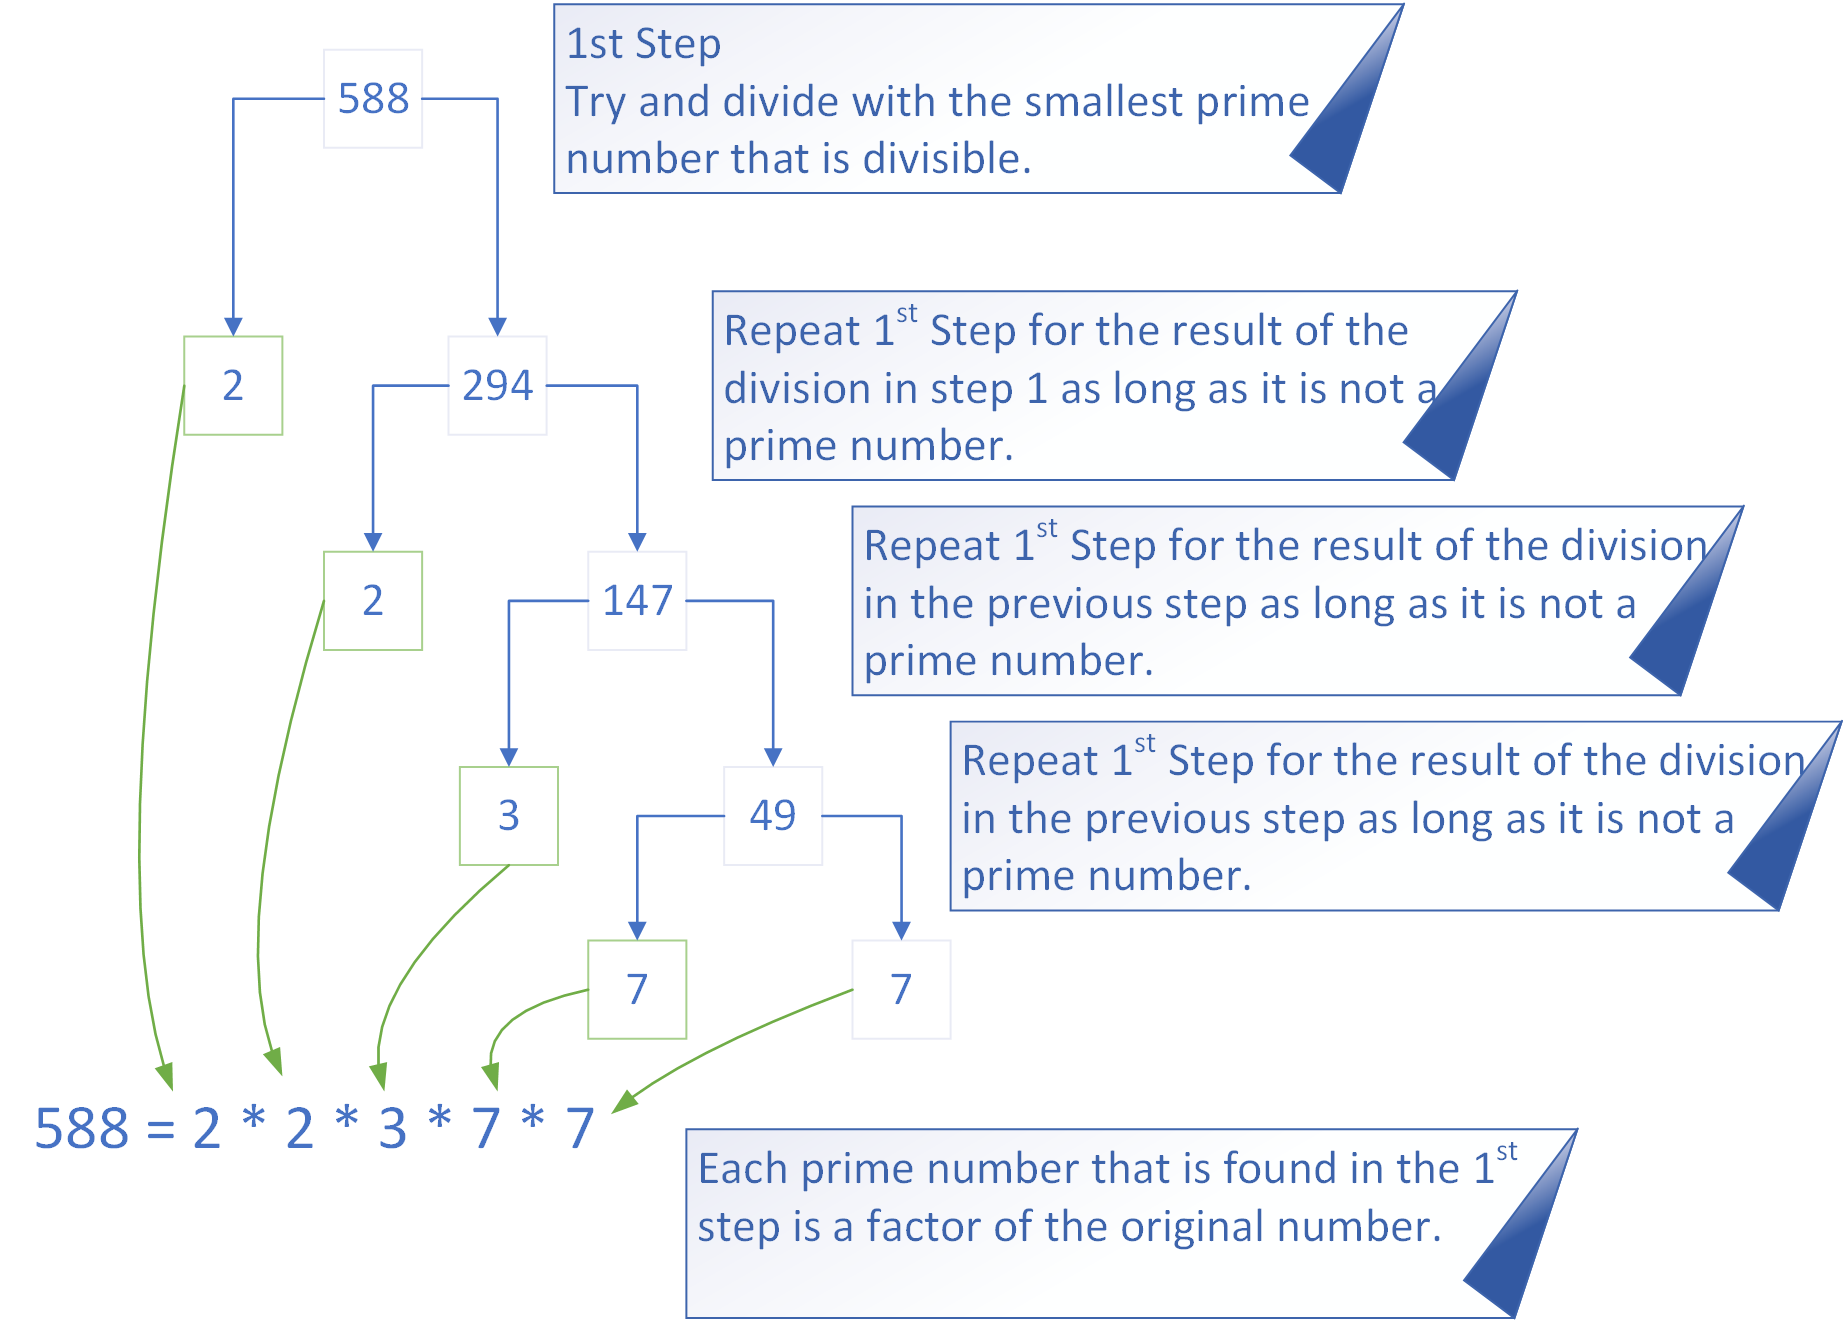
\includegraphics[width=1\linewidth]{images/factorisation_1} 

}

\caption{Prime Factorisation of 588}\label{fig:unnamed-chunk-6}
\end{figure}

\hypertarget{lcm-and-hcf}{%
\section{LCM and HCF}\label{lcm-and-hcf}}

Imagine you are a self employed software developer and you have a carpenter as a costumer. Your costumer wants an online web page together with a database store and online tools to help him with selecting wood sizes. The carpenter receives large pieces of wood of various sizes but he always ends up with a large amount of waste that sometimes he does not have the space to store. They want a tool to help them out with finding the best combination of what sizes of wood would be required that could be cut in equal lengths by producing the minimum waste.
They also require to organise their wood delivery a bit better, as they would want the delivery from different suppliers to happen at different times.

To solve the first part of the above problem one would need to find a common size between the pieces of wood that they already have in order to be able to cut them in equal strips.

To solve the second part of the above problem one would need to find the how ofter that deliveries from different suppliers happen.

Both of these problems can be partly solved by using what in mathematics is called the highest common factor (HCF) and the lowest common multiple (LCM).

\hypertarget{hcf}{%
\subsection{HCF}\label{hcf}}

HCF can also be called with the names Greatest Common Measure(GCM) and Greatest Common Divisor(GCD).The HCF is the largest natural number that divides evenly into all numbers with zero remainder.

The usual usage in real life is for helping us divide things into smaller sections. To arrange data or anything into rows and groups.

For example, for the set of numbers 18 and 12 the GCF(18,12) = 6. So 6 is the largest natural number that divides both 18 and 12 that produces a natural number.

\hypertarget{lcm}{%
\subsection{LCM}\label{lcm}}

LCM can also be called with the names least common multiple or smallest common multiple (SCM). The LCM is the smallest natural number that is evenly divisible between multiple numbers.

The usual usage in real life is for helping us find repeated events, to help us order enough material to satisfy manufacturing over a period of time and also to find when multiple repeatable events would coincide.

A simple example would be the LCM(2,3) = 6. So 6 is the smallest natural number that can be divided by both 2 and 3 that produces a natural number.

A multiple of an integer (whole number) is any integer that appears in its times table. For example, the multiples of 3 are 3, 6, 9, 12, and so on.

A factor of an integer is any integer that divides the integer with no remainder. For example, the factors of 36 are 1, 2, 3, 4, 6, 9, 12, 18, and 36.

\hypertarget{calculation-of-hcf-and-lcm}{%
\subsection{Calculation of HCF and LCM}\label{calculation-of-hcf-and-lcm}}

The first step to calculate HCF or LCM is to perform prime factorisation of each number.

Once you have completed the factorisation of each number HCF and LCM can be calculated.

To find HCF find all the similar prime factors of each factorisation and multiply them together.

To find LCM find for each prime number the largest presence of each factorisation and multiply them.

Let us see an example:

\begin{figure}

{\centering 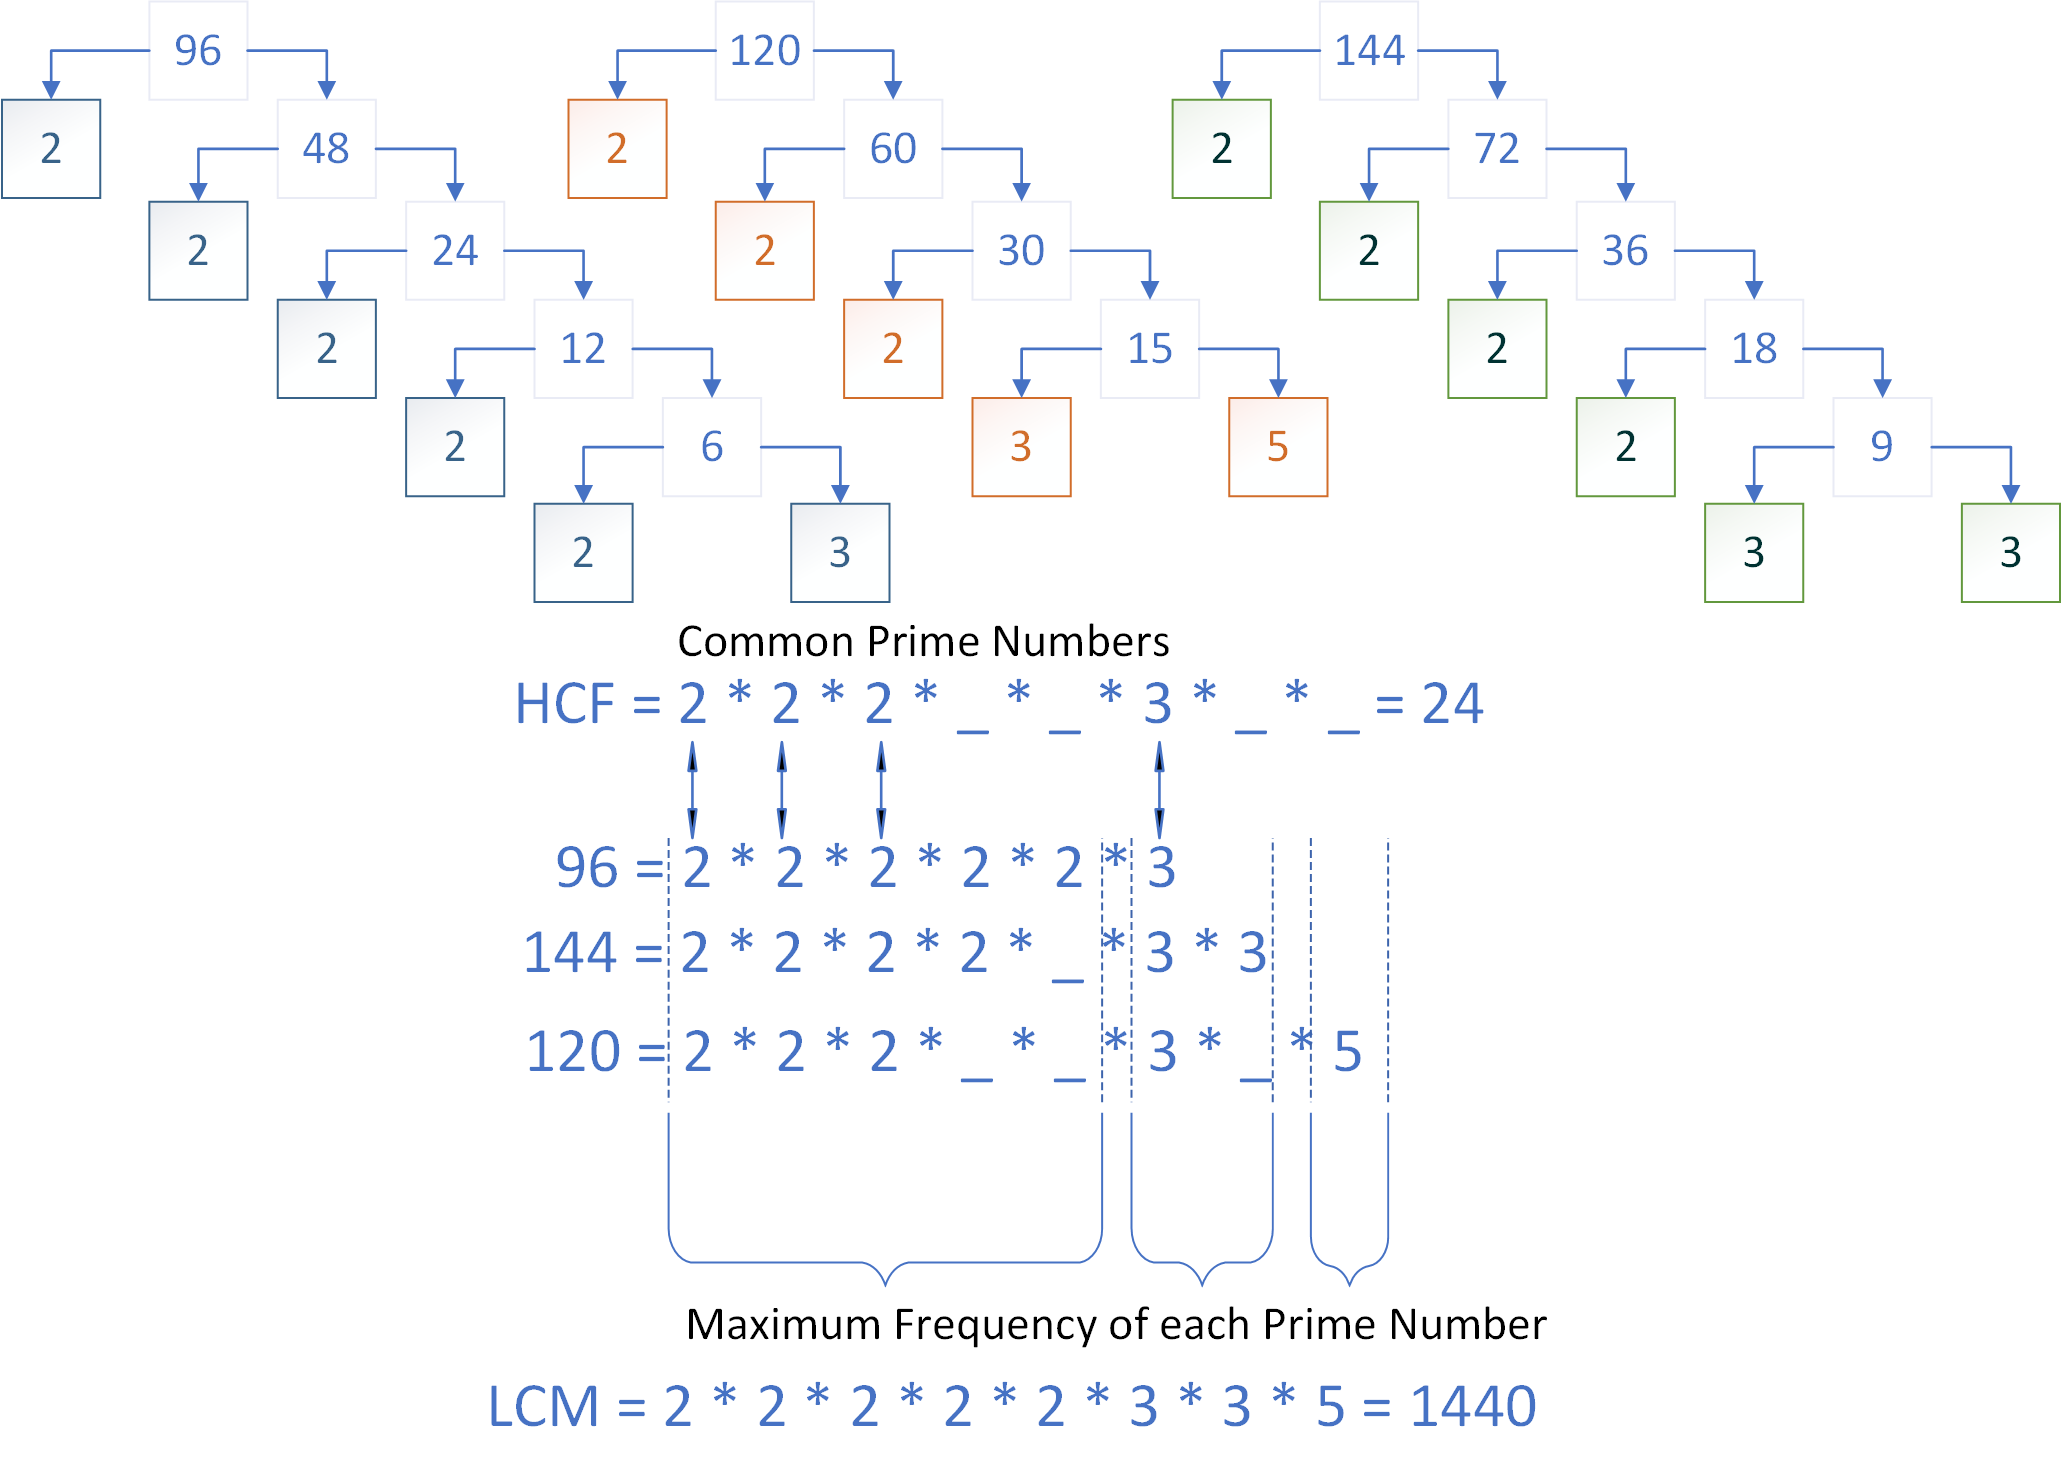
\includegraphics[width=1\linewidth]{images/HCF_LCM} 

}

\caption{HRF and LCM Calculation for three numbers}\label{fig:unnamed-chunk-7}
\end{figure}

In the example to find HCF you need to find where all prime factors appear on the same column and then multiply them.
For LCM you find the maximum times a prime factor is being used and multiply them together.

\hypertarget{fractions}{%
\section{Fractions}\label{fractions}}

\hypertarget{decimals}{%
\section{Decimals}\label{decimals}}

\hypertarget{percentages}{%
\section{Percentages}\label{percentages}}

\hypertarget{rounding-numbers}{%
\section{Rounding Numbers}\label{rounding-numbers}}

\hypertarget{standard-form}{%
\section{Standard Form}\label{standard-form}}

\hypertarget{excersises}{%
\section{Excersises}\label{excersises}}

\hypertarget{algebra-basics}{%
\chapter{Algebra -- Basics}\label{algebra-basics}}

\hypertarget{powers-and-roots}{%
\section{Powers and roots}\label{powers-and-roots}}

\hypertarget{expanding-brackets}{%
\section{Expanding Brackets}\label{expanding-brackets}}

\hypertarget{factorising}{%
\section{Factorising}\label{factorising}}

\hypertarget{manipulating-surds}{%
\section{Manipulating Surds}\label{manipulating-surds}}

\hypertarget{algebra-quadratics-and-simultaneous-equations}{%
\chapter{Algebra -- Quadratics and Simultaneous Equations}\label{algebra-quadratics-and-simultaneous-equations}}

\hypertarget{solving-and-rearranging-equations}{%
\section{Solving and rearranging Equations}\label{solving-and-rearranging-equations}}

\hypertarget{factorising-quadratics}{%
\section{Factorising quadratics}\label{factorising-quadratics}}

\hypertarget{quadratic-formula}{%
\section{Quadratic Formula}\label{quadratic-formula}}

\hypertarget{algebraic-fractions}{%
\section{Algebraic Fractions}\label{algebraic-fractions}}

\hypertarget{sequences}{%
\section{Sequences}\label{sequences}}

\hypertarget{inequalities}{%
\section{Inequalities}\label{inequalities}}

\hypertarget{simultaneous-equations}{%
\section{Simultaneous Equations}\label{simultaneous-equations}}

\hypertarget{geometry-and-thinking}{%
\chapter{Geometry and thinking}\label{geometry-and-thinking}}

\hypertarget{rules-of-geometry}{%
\section{Rules of Geometry}\label{rules-of-geometry}}

\hypertarget{parallel-lines}{%
\section{Parallel lines}\label{parallel-lines}}

\hypertarget{angles}{%
\section{Angles}\label{angles}}

\hypertarget{properties-of-known-geometrical-shapes}{%
\section{Properties of known geometrical shapes}\label{properties-of-known-geometrical-shapes}}

\hypertarget{circle}{%
\section{Circle}\label{circle}}

\hypertarget{transformation}{%
\section{Transformation}\label{transformation}}

\hypertarget{areas}{%
\section{Areas}\label{areas}}

\hypertarget{scale-factors}{%
\section{Scale Factors}\label{scale-factors}}

\hypertarget{graphs-and-coordinate-geometry}{%
\chapter{Graphs and Coordinate Geometry}\label{graphs-and-coordinate-geometry}}

\hypertarget{polynomials}{%
\section{Polynomials}\label{polynomials}}

\hypertarget{probability-and-statistics}{%
\chapter{Probability and Statistics}\label{probability-and-statistics}}

\hypertarget{probability-basics}{%
\section{Probability basics}\label{probability-basics}}

\hypertarget{counting-outcomes}{%
\section{Counting Outcomes}\label{counting-outcomes}}

\hypertarget{tree-diagrams}{%
\section{Tree Diagrams}\label{tree-diagrams}}

\hypertarget{sets-and-venn-diagrams}{%
\section{Sets and Venn Diagrams}\label{sets-and-venn-diagrams}}

\hypertarget{sampling-and-data-collection}{%
\section{Sampling and Data collection}\label{sampling-and-data-collection}}

\hypertarget{mean-median-mode-and-range}{%
\section{Mean, Median, Mode and range}\label{mean-median-mode-and-range}}

\hypertarget{frequency-tables}{%
\section{Frequency tables}\label{frequency-tables}}

\hypertarget{plots}{%
\section{Plots}\label{plots}}

\hypertarget{polynomials-1}{%
\chapter{Polynomials}\label{polynomials-1}}

\hypertarget{logarithms-and-exponentials}{%
\chapter{Logarithms and Exponentials}\label{logarithms-and-exponentials}}

\hypertarget{introduction-to-discrete-mathematics}{%
\chapter{Introduction to Discrete mathematics}\label{introduction-to-discrete-mathematics}}

\hypertarget{intro}{%
\chapter{Introduction}\label{intro}}

Welcome to Advance Mathematics Module (MCOMD0AMA). This module will cover material from GCSE to A Level maths, that is relevant and required for any computing course in this University.

These pages are comprised of theory and excersises to h

You can label chapter and section titles using \texttt{\{\#label\}} after them, e.g., we can reference Chapter \ref{intro}. If you do not manually label them, there will be automatic labels anyway, e.g., Chapter \ref{methods}.

Figures and tables with captions will be placed in \texttt{figure} and \texttt{table} environments, respectively.

\begin{Shaded}
\begin{Highlighting}[]
\KeywordTok{par}\NormalTok{(}\DataTypeTok{mar =} \KeywordTok{c}\NormalTok{(}\DecValTok{4}\NormalTok{, }\DecValTok{4}\NormalTok{, }\FloatTok{.1}\NormalTok{, }\FloatTok{.1}\NormalTok{))}
\KeywordTok{plot}\NormalTok{(pressure, }\DataTypeTok{type =} \StringTok{'b'}\NormalTok{, }\DataTypeTok{pch =} \DecValTok{19}\NormalTok{)}
\end{Highlighting}
\end{Shaded}

\begin{figure}

{\centering 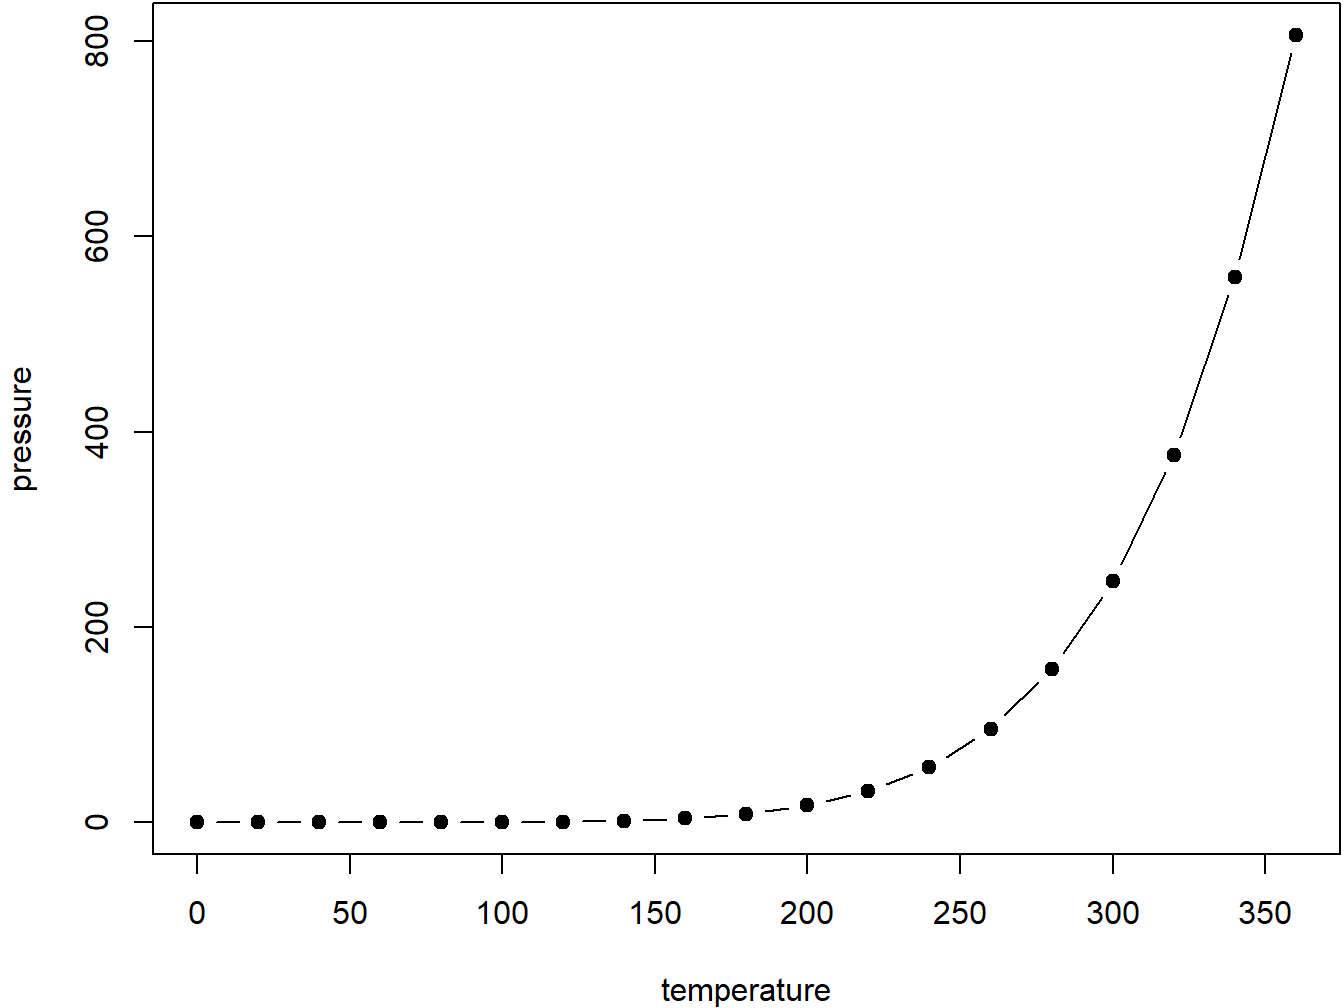
\includegraphics[width=0.8\linewidth]{MCOMD0AMA_files/figure-latex/nice-fig-1} 

}

\caption{Here is a nice figure!}\label{fig:nice-fig}
\end{figure}

Reference a figure by its code chunk label with the \texttt{fig:} prefix, e.g., see Figure \ref{fig:nice-fig}. Similarly, you can reference tables generated from \texttt{knitr::kable()}, e.g., see Table \ref{tab:nice-tab}.

\begin{Shaded}
\begin{Highlighting}[]
\NormalTok{knitr}\OperatorTok{::}\KeywordTok{kable}\NormalTok{(}
  \KeywordTok{head}\NormalTok{(iris, }\DecValTok{20}\NormalTok{), }\DataTypeTok{caption =} \StringTok{'Here is a nice table!'}\NormalTok{,}
  \DataTypeTok{booktabs =} \OtherTok{TRUE}
\NormalTok{)}
\end{Highlighting}
\end{Shaded}

\begin{table}

\caption{\label{tab:nice-tab}Here is a nice table!}
\centering
\begin{tabular}[t]{rrrrl}
\toprule
Sepal.Length & Sepal.Width & Petal.Length & Petal.Width & Species\\
\midrule
5.1 & 3.5 & 1.4 & 0.2 & setosa\\
4.9 & 3.0 & 1.4 & 0.2 & setosa\\
4.7 & 3.2 & 1.3 & 0.2 & setosa\\
4.6 & 3.1 & 1.5 & 0.2 & setosa\\
5.0 & 3.6 & 1.4 & 0.2 & setosa\\
\addlinespace
5.4 & 3.9 & 1.7 & 0.4 & setosa\\
4.6 & 3.4 & 1.4 & 0.3 & setosa\\
5.0 & 3.4 & 1.5 & 0.2 & setosa\\
4.4 & 2.9 & 1.4 & 0.2 & setosa\\
4.9 & 3.1 & 1.5 & 0.1 & setosa\\
\addlinespace
5.4 & 3.7 & 1.5 & 0.2 & setosa\\
4.8 & 3.4 & 1.6 & 0.2 & setosa\\
4.8 & 3.0 & 1.4 & 0.1 & setosa\\
4.3 & 3.0 & 1.1 & 0.1 & setosa\\
5.8 & 4.0 & 1.2 & 0.2 & setosa\\
\addlinespace
5.7 & 4.4 & 1.5 & 0.4 & setosa\\
5.4 & 3.9 & 1.3 & 0.4 & setosa\\
5.1 & 3.5 & 1.4 & 0.3 & setosa\\
5.7 & 3.8 & 1.7 & 0.3 & setosa\\
5.1 & 3.8 & 1.5 & 0.3 & setosa\\
\bottomrule
\end{tabular}
\end{table}

You can write citations, too. For example, we are using the \textbf{bookdown} package \citep{R-bookdown} in this sample book, which was built on top of R Markdown and \textbf{knitr} \citep{xie2015}.

  \bibliography{book.bib,packages.bib}

\end{document}
